 \documentclass[11pt]{article}


\usepackage{soul}
\usepackage{natbib}
\usepackage{hyperref}
\usepackage{bookmark}
\usepackage{graphicx}             
\graphicspath{{./Figuras/}}

\usepackage{makecell}
\usepackage[margin=1in]{geometry}
\usepackage{float}                
\usepackage{amsmath}
\usepackage{amscd}
\usepackage{amsfonts}
\usepackage{amssymb}
\usepackage{bbm}
\usepackage{booktabs}
\usepackage{nameref}
\usepackage{multirow}
\usepackage[nokeyprefix]{refstyle}
\usepackage{rotating}
\usepackage{threeparttable}
\usepackage{afterpage}
\usepackage{lscape}
\usepackage{enumerate}
\usepackage{caption}
\usepackage{subcaption}
\usepackage{epstopdf}
\usepackage{setspace}
\usepackage{svg}
\usepackage{dsfont}
\usepackage{amsthm}
\usepackage{tocloft}
\usepackage{etoc}
\usepackage{lmodern}
\usepackage{bm}

\epstopdfDeclareGraphicsRule{.tiff}{png}{.png}{convert #1 \OutputFile}
\AppendGraphicsExtensions{.tiff}

\epstopdfDeclareGraphicsRule{.tif}{png}{.png}{convert #1 \OutputFile}
\AppendGraphicsExtensions{.tif}

\usepackage{tikz}
\usetikzlibrary{shapes.geometric, arrows}
\usetikzlibrary{calc}
\usetikzlibrary{matrix}

\tikzset{ 
    table/.style={
        matrix of nodes,
        row sep=-\pgflinewidth,
        column sep=-\pgflinewidth,
        nodes={
            rectangle,
            draw=black,
            align=center
        },
        minimum height=1.5em,
        text depth=0.5ex,
        text height=2ex,
        nodes in empty cells,
%%
        every even row/.style={
            nodes={fill=gray!20}
        },
        column 1/.style={
            nodes={text width=2em,font=\bfseries}
        },
        row 1/.style={
            nodes={
                fill=black,
                text=white,
                font=\bfseries
            }
        }
    }
}


\usepackage{colortbl}

\newtheorem{theorem}{Theorem}
\newtheorem{claim}[theorem]{Claim}
\newtheorem{prop}[theorem]{Proposition} 
\newtheorem{cor}[theorem]{Corollary} 

\DeclareRobustCommand{\hlgr}[1]{{\sethlcolor{green}\hl{#1}}}


\usepackage{comment}
%para esconder columnas en tablas (enrique)
\usepackage{array}
\newcolumntype{H}{>{\setbox0=\hbox\bgroup}c<{\egroup}@{}}
\linespread{1.25}

\newcommand{\wh}{\widehat}
\usepackage{anyfontsize}

\usepackage[linesnumbered,vlined,ruled,commentsnumbered]{algorithm2e}

\DontPrintSemicolon
\newcommand{\To}{\mbox{\upshape\bfseries to}}
\usepackage{anyfontsize}
%%% HELPER CODE FOR DEALING WITH EXTERNAL REFERENCES
\usepackage{xr}
\makeatletter
\newcommand*{\addFileDependency}[1]{
  \typeout{(#1)}
  \@addtofilelist{#1}
  \IfFileExists{#1}{}{\typeout{No file #1.}}
}
\makeatother

\newcommand*{\myexternaldocument}[1]{
    \externaldocument{#1}
    \addFileDependency{#1.tex}
    \addFileDependency{#1.aux}
}

%\myexternaldocument{OA}

%%%%%%%%%%%%%%%%%%%%%%%%%%%%%%%% DOCUMENT
\begin{document}


\title{Frequent Payment \thanks{}}
\author{Joyce Sadka \and Enrique Seira  }
\date{This draft:  \today \\[2 cm]}

%\vspace{.5in}


\maketitle
\begin{abstract}
XXX 
\end{abstract}

\textbf{Keywords: } XXX.

\textbf{XXX} XXX

\newpage



\section{Introduction}


\section{Conclusion}





%%%%%%%%%%%%%%%%%%%%%%%%%%%%%%%%%%%%%%%%%%%%%%%%%%%%%%%%%%%%%



\pagebreak
%%%%%%%%%%%%%%%%%%%%%%%%%%%%%%%%%%%%%%%%%%%%%%%%%%%%%%%%%%%%%
%BIBLIOGRAPHY




\section{Tables}


\begin{table}[H]
\caption{Summary statistics}
\label{SS}
\begin{center}
\scriptsize{% Table generated by Excel2LaTeX from sheet 'SS'
\begin{tabular}{lcccccccc}
\toprule
      &       &       & \multicolumn{5}{c}{Treatment arms}    &  \\
\midrule
      &       &       &       & \multicolumn{2}{c}{No Choice } & \multicolumn{2}{c}{Choice} &  \\
\midrule
\midrule
      & Overall & Pre-experiment & Control & Fee   & Promise & Fee   & Promise & p-value \\
\midrule
      & \multicolumn{8}{c}{Panel A : Administrative Data} \\
\midrule
\midrule
Loan amount  & 2197  & 2239  & 2301  & 2147  & 2133  & 2181  & 2089  & 0.32 \\
      & (25)  & (39)  & (79)  & (72)  & (74)  & (65)  & (65)  &  \\
Monday & 0.18  & 0.16  & 0.18  & 0.16  & 0.17  & 0.19  & 0.21  & 0.96 \\
      & (0.02) & (0.03) & (0.05) & (0.05) & (0.06) & (0.06) & (0.05) &  \\
Number of branch-day pawns & 34    & 36    & 31    & 31    & 32    & 37    & 34    & 0.38 \\
      & (0.82) & (1.25) & (2.2) & (2.35) & (2.38) & (2.65) & (1.76) &  \\
\midrule
Number of branch-days & -     &       & 84    & 80    & 68    & 93    & 82    &  \\
Obs   & 21808 & 8366  & 2601  & 2484  & 2156  & 3435  & 2766  &  \\
\midrule
      & \multicolumn{8}{c}{Panel B : Survey Data (conditional on pawning)} \\
\midrule
\midrule
Woman & 0.73  &       & 0.76  & 0.72  & 0.73  & 0.72  & 0.74  & 0.41 \\
      & (0.01) &       & (0.02) & (0.02) & (0.02) & (0.02) & (0.01) &  \\
Age   & 43.31 &       & 43.16 & 43.17 & 42.96 & 43.96 & 43.06 & 0.79 \\
      & (0.28) &       & (0.57) & (0.79) & (0.65) & (0.61) & (0.52) &  \\
Subjective value & 3068  &       & 3151  & 2978  & 2985  & 3114  & 3079  & 0.41 \\
      & (39)  &       & (69)  & (91)  & (76)  & (85)  & (100) &  \\
Has pawn before & 0.9   &       & 0.89  & 0.9   & 0.89  & 0.91  & 0.89  & 0.68 \\
      & (0)   &       & (0.01) & (0.01) & (0.01) & (0.01) & (0.01) &  \\
Subj. pr. of recovery & 93.14 &       & 92.74 & 92.16 & 93.6  & 93.67 & 93.3  & 0.46 \\
      & (0)   &       & (0.55) & (0.86) & (0.6) & (0.47) & (0.6) &  \\
+High-school & 0.66  &       & 0.66  & 0.67  & 0.65  & 0.67  & 0.64  & 0.74 \\
      & (0.01) &       & (0.02) & (0.02) & (0.02) & (0.02) & (0.02) &  \\
Survey response rate & 0.78  &       & 0.77  & 0.75  & 0.8   & 0.77  & 0.79  & 0.5 \\
      & (0.01) &       & (0.02) & (0.03) & (0.02) & (0.02) & (0.02) &  \\
\midrule
Obs   & 10431 &       & 2000  & 1855  & 1732  & 2652  & 2192  &  \\
\midrule
\midrule
      & \multicolumn{8}{c}{Panel C : Survey Data (unconditional)} \\
\midrule
\midrule
Woman & 0.74  & 0.75  & 0.76  & 0.72  & 0.73  & 0.72  & 0.74  & 0.32 \\
      & (0.01) & (0.01) & (0.02) & (0.02) & (0.02) & (0.02) & (0.01) &  \\
Age   & 43.24 & 43.06 & 43.2  & 43.21 & 43.01 & 44.07 & 43.07 & 0.79 \\
      & (0.21) & (0.32) & (0.56) & (0.77) & (0.66) & (0.61) & (0.51) &  \\
Subjective value & 3112  & 3192  & 3145  & 2985  & 3010  & 3111  & 3082  & 0.41 \\
      & (36)  & (75)  & (68)  & (88)  & (76)  & (84)  & (99)  &  \\
Has pawn before & 0.89  & 0.88  & 0.89  & 0.9   & 0.89  & 0.91  & 0.89  & 0.56 \\
      & (0.01) & (0.01) & (0.01) & (0.01) & (0.01) & (0.01) & (0.01) &  \\
Subj. pr. of recovery & 92.64 & 91.84 & 92.73 & 92.19 & 93.66 & 93.71 & 93.34 & 0 \\
      & (0.2) & (0.31) & (0.54) & (0.84) & (0.59) & (0.46) & (0.59) &  \\
+High-school & 0.63  & 0.6   & 0.66  & 0.67  & 0.65  & 0.66  & 0.64  & 0.01 \\
      & (0.01) & (0.01) & (0.02) & (0.02) & (0.02) & (0.02) & (0.02) &  \\
\% ended up pawning &       &       & 0.98  & 0.97  & 0.99  & 0.98  & 0.99  & 0.25 \\
\midrule
Obs   & 17546 & 6919  & 2035  & 1907  & 1757  & 2710  & 2218  &  \\
\bottomrule
\bottomrule
\end{tabular}%
}
\end{center}
 \footnotesize
\textit{Notes:} 

\textit{Do file: } \texttt{ss.do}
\end{table}




\pagebreak




%%%%%%%%%%%%%%%%%%%%%%%%%%%%%%%%%%%%%%%%%%%%%%%%%%%%%%

\section{Figures}


\begin{figure}[H]
        \caption{Timeline of the experiment}
    \label{micas}
    \begin{center}
        \centering
        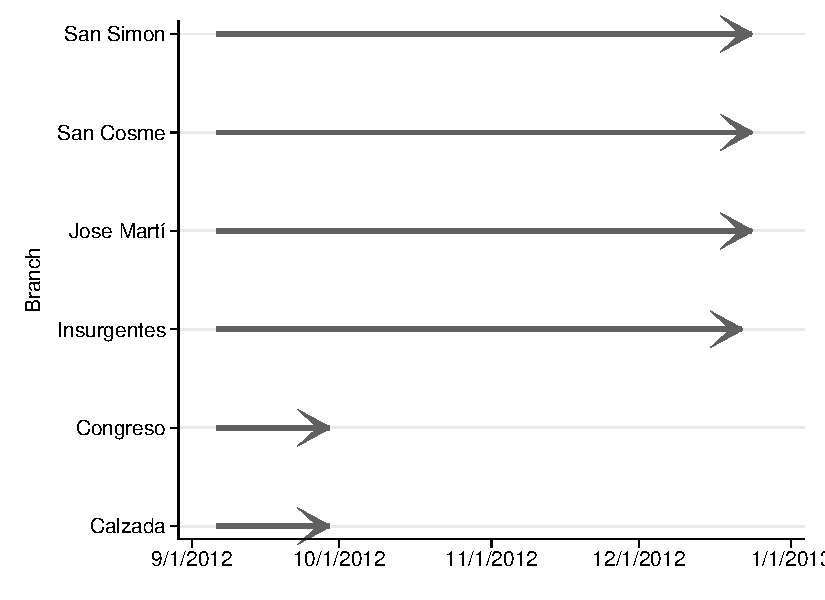
\includegraphics[width=0.70\textwidth]{Figuras/timeline_suc_exp.pdf}
    \end{center}
     \footnotesize \textit{Notes: } 
      \footnotesize{ \textit{Do file: }  \texttt{timeline\_suc\_exp.do}}
\end{figure}


\begin{figure}[H]
        \caption{Experiment arms}
    \label{micas}
    \begin{center}
        \centering
        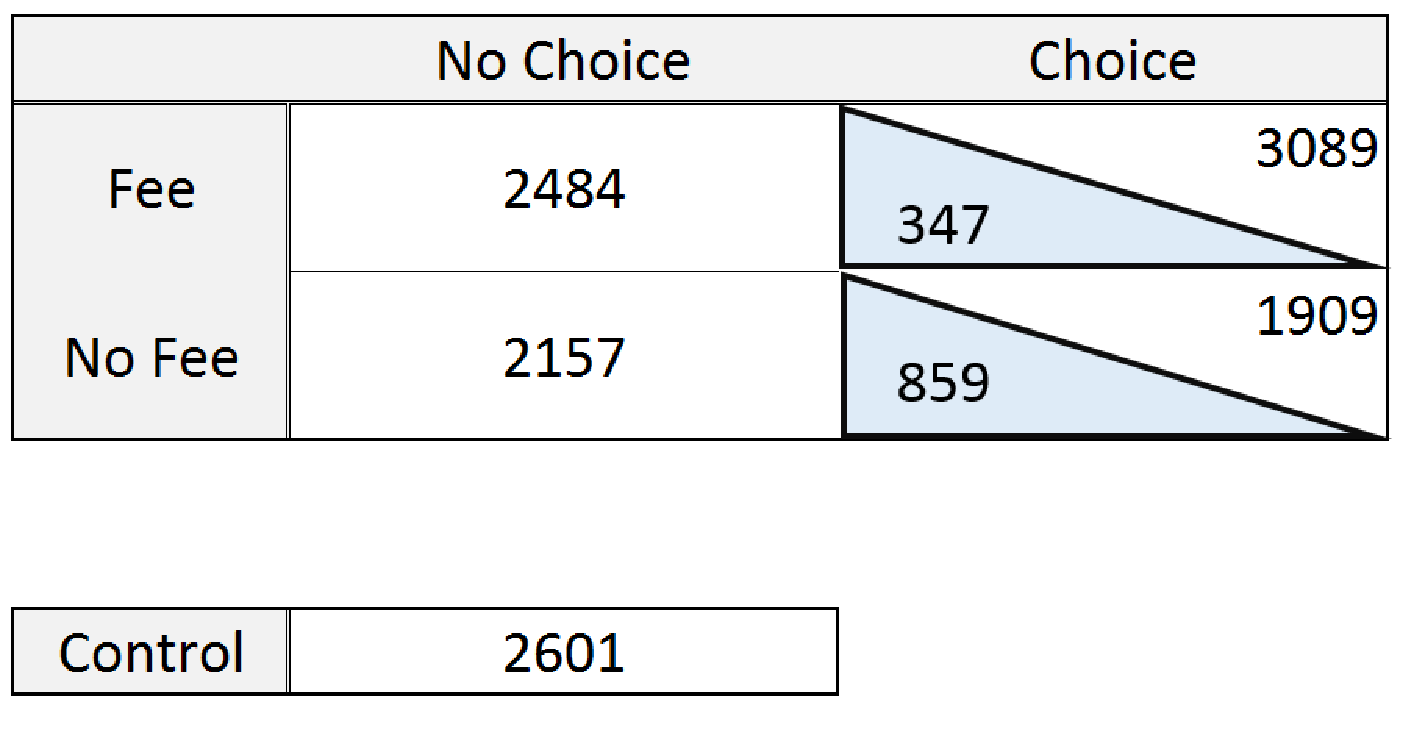
\includegraphics[width=0.70\textwidth]{Figuras/exp_arms.pdf}
    \end{center}
     \footnotesize \textit{Notes: } 
      \footnotesize{ }
\end{figure}


\begin{figure}[H]
        \caption{Booklet with product information}
    \label{micas}
    \begin{center}
        \centering
        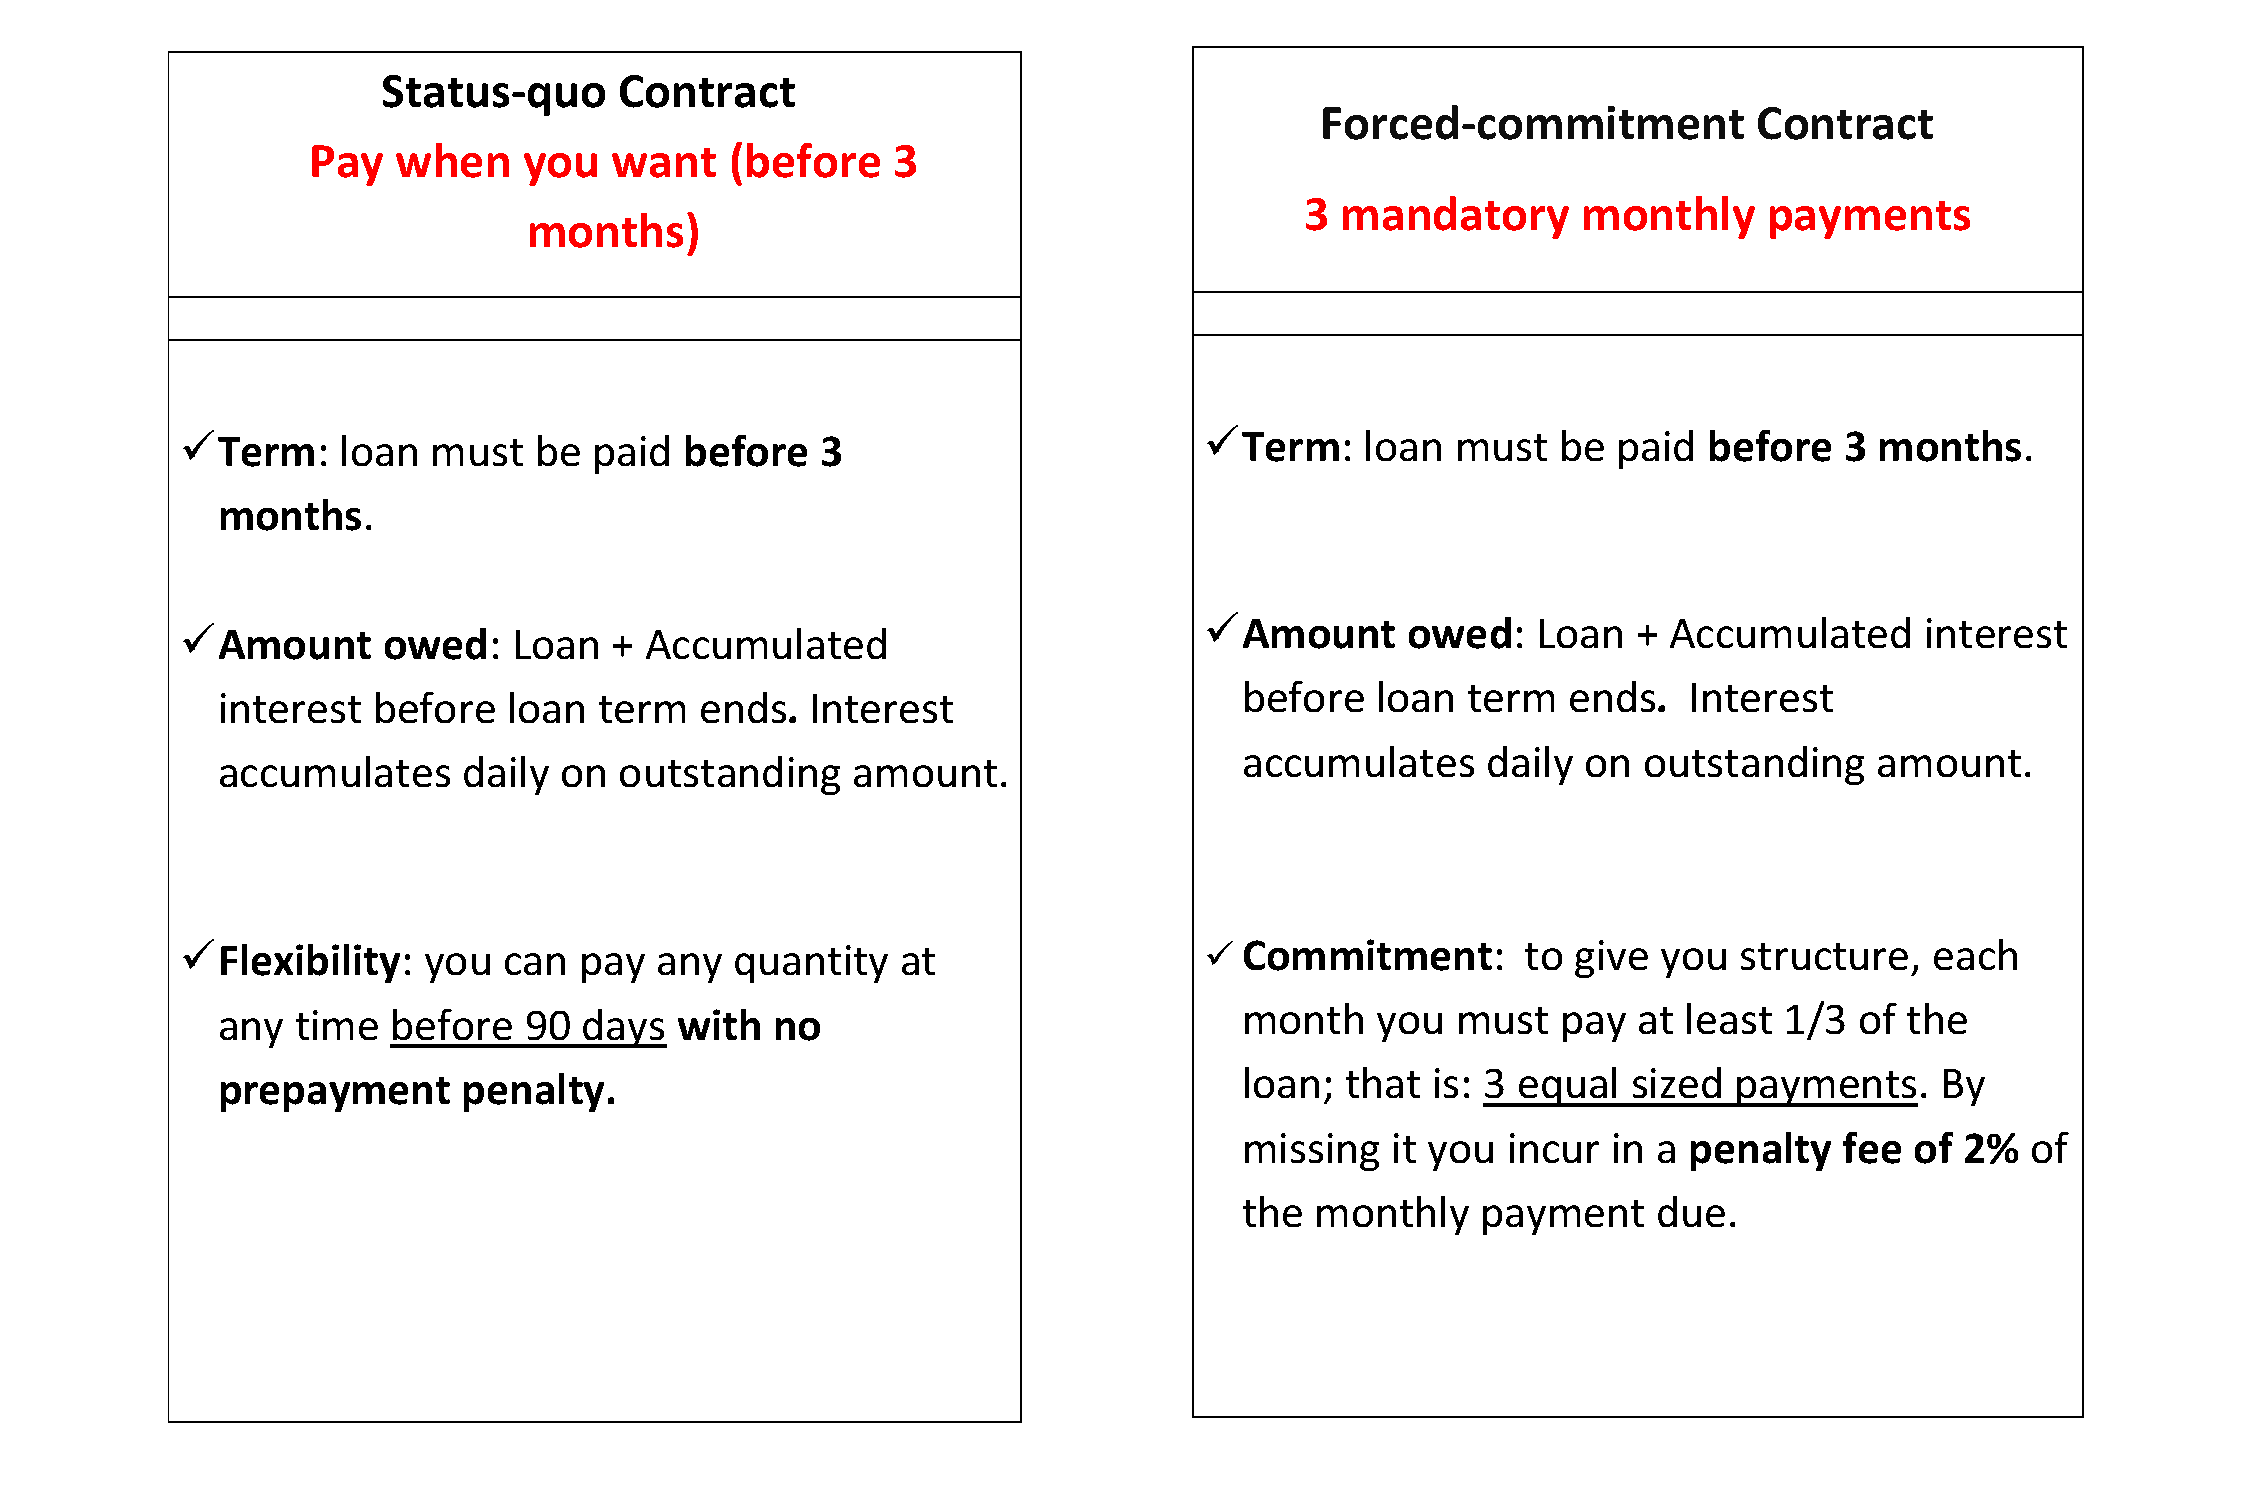
\includegraphics[width=\textwidth]{micas.pdf}
    \end{center}
     \footnotesize \textit{Notes: } 
      \footnotesize{ }
\end{figure}


\begin{figure}[H]
    \caption{Treatment Effect}
    \label{Treatment Effect}
    \begin{center}
    \begin{subfigure}{0.4\textwidth}
        \caption{Paid loan}
        \centering
        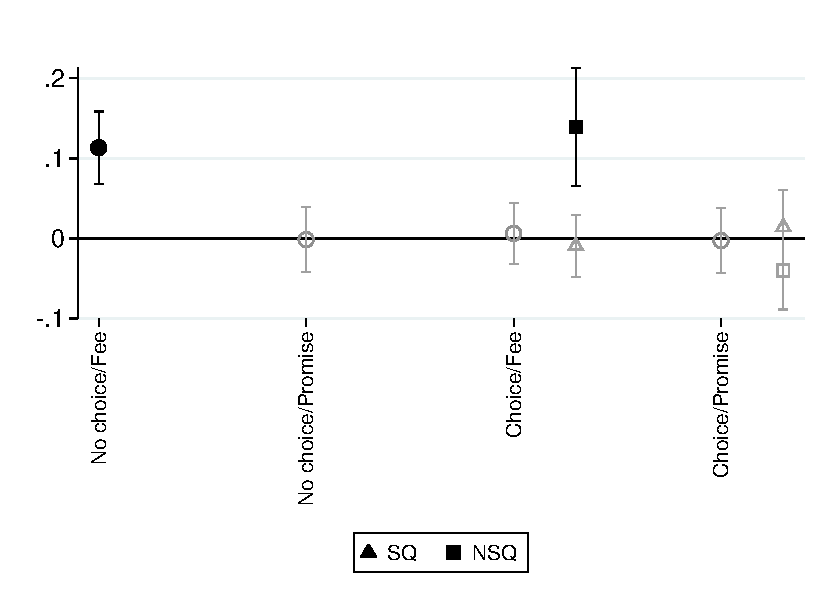
\includegraphics[width=\textwidth]{Figuras/te_graph_des_c.pdf}
    \end{subfigure}
    \begin{subfigure}{0.4\textwidth}
        \caption{Number of payments}
        \centering
        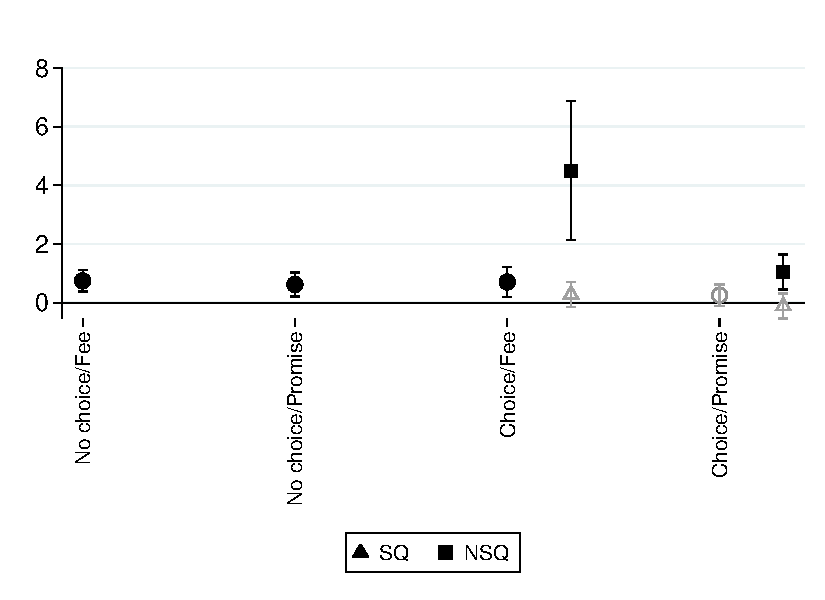
\includegraphics[width=\textwidth]{Figuras/te_graph_num_p.pdf}
    \end{subfigure}
     \begin{subfigure}{0.4\textwidth}
      \caption{Percentage of payment}
        \centering
        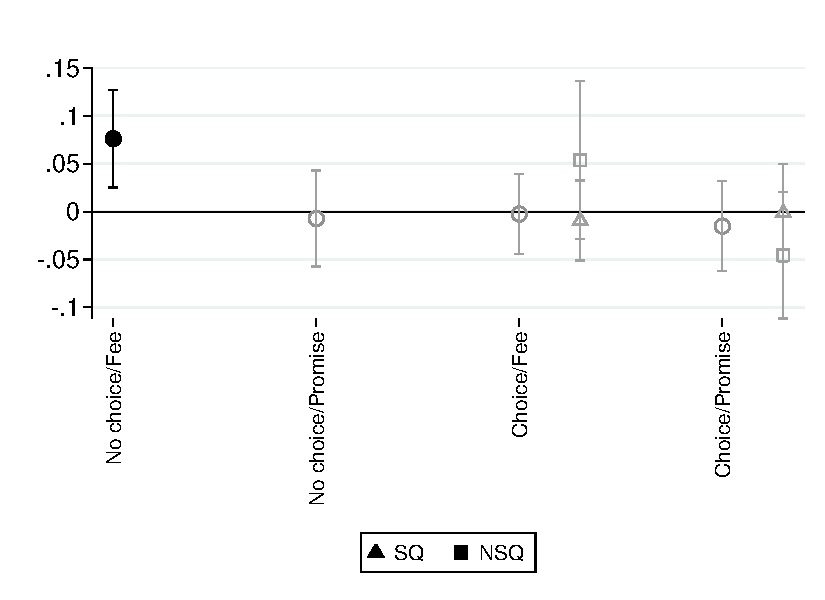
\includegraphics[width=\textwidth]{Figuras/te_graph_sum_porcp_c.pdf}
    \end{subfigure}
      \begin{subfigure}{0.4\textwidth}
      \caption{Days to un-pledge}
        \centering
        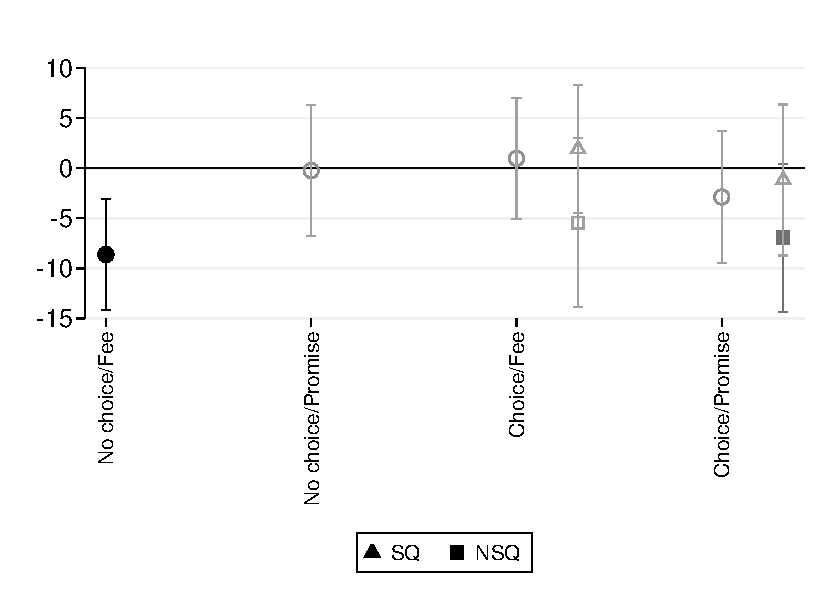
\includegraphics[width=\textwidth]{Figuras/te_graph_dias_al_desempenyo.pdf}
    \end{subfigure}
    \end{center}
     \footnotesize \textit{Notes: } 
      \footnotesize{ \textit{Do file: }  \texttt{te.do}}
\end{figure}

\begin{figure}[H]
        \caption{Reincidence}
    \label{micas}
    \begin{center}
        \centering
        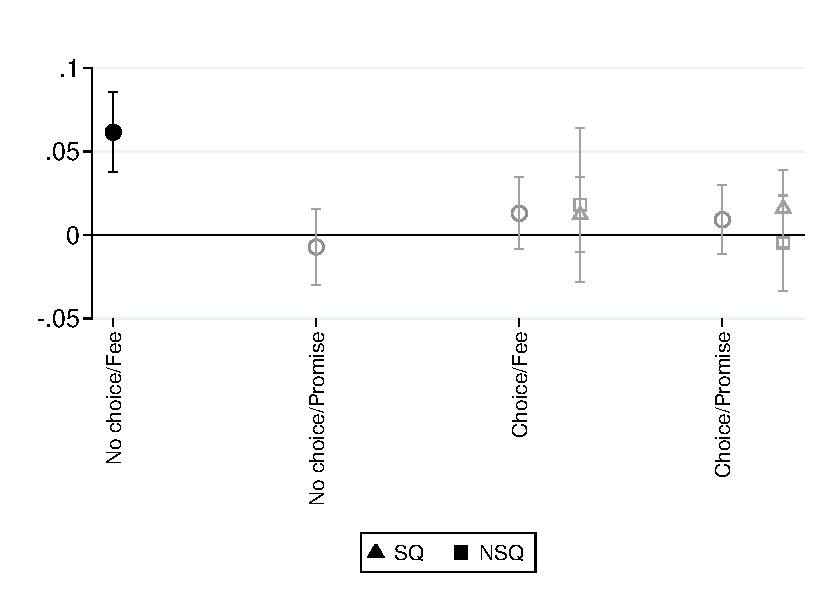
\includegraphics[width=\textwidth]{Figuras/te_graph_reincidence.pdf}
    \end{center}
     \footnotesize \textit{Notes: } 
      \footnotesize{ }
\end{figure}


\begin{figure}[H]
    \caption{Heterogeneous Treatment Effect}
    \label{Treatment Effect}
    \begin{center}
    \begin{subfigure}{0.4\textwidth}
        \caption{Paid loan}
        \centering
        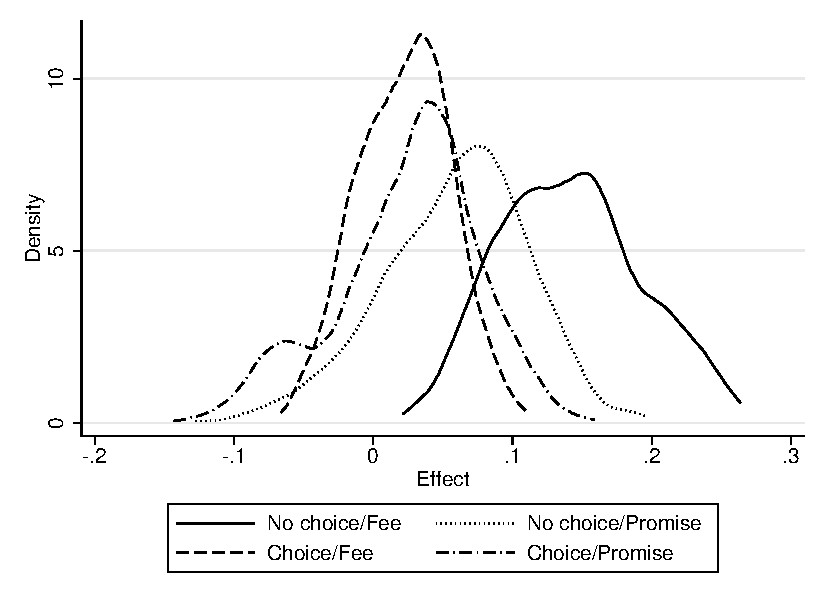
\includegraphics[width=\textwidth]{Figuras/he_dist_des_c.pdf}
    \end{subfigure}
    \begin{subfigure}{0.4\textwidth}
        \caption{Number of payments}
        \centering
        \includegraphics[width=\textwidth]{Figuras/he_dist_num_p.pdf}
    \end{subfigure}
     \begin{subfigure}{0.4\textwidth}
      \caption{Percentage of payment}
        \centering
        \includegraphics[width=\textwidth]{Figuras/he_dist_sum_porcp_c.pdf}
    \end{subfigure}
    \begin{subfigure}{0.4\textwidth}
      \caption{Days to un-pledge}
        \centering
        \includegraphics[width=\textwidth]{Figuras/he_dist_dias_al_desempenyo.pdf}
    \end{subfigure}    
    \end{center}
     \footnotesize \textit{Notes: } 
      \footnotesize{ \textit{Do file: }  \texttt{te.do}}
\end{figure}



\begin{figure}[H]
        \caption{Histogram of payments}
    \label{HistPayments}
    \begin{center}
        \centering
        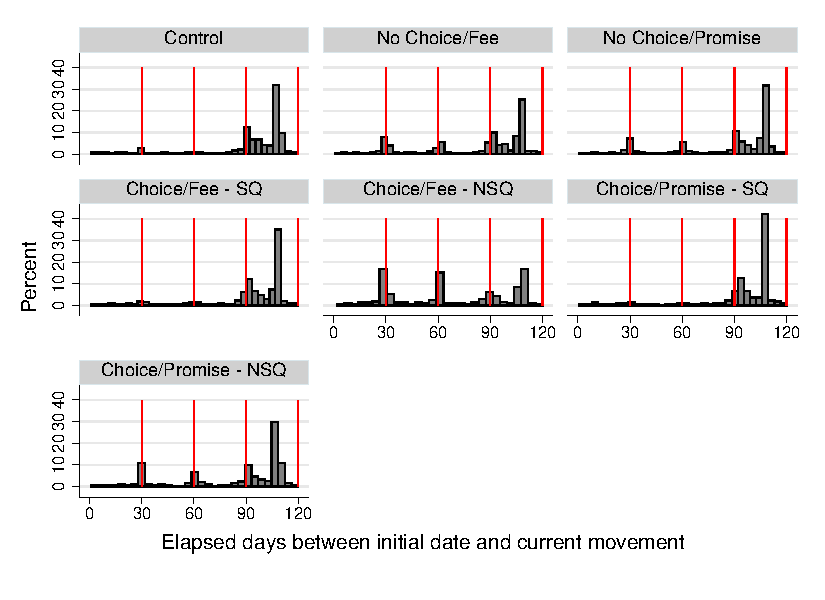
\includegraphics[width=\textwidth]{hist_payments.pdf}
    \end{center}
     \footnotesize \textit{Notes: } 
      \footnotesize{ \textit{Do file: }  \texttt{hist\_payments.do}}
\end{figure}


\begin{figure}[H]
        \caption{Percentage of payments}
    \label{HistPayments}
    \begin{center}
        \centering
        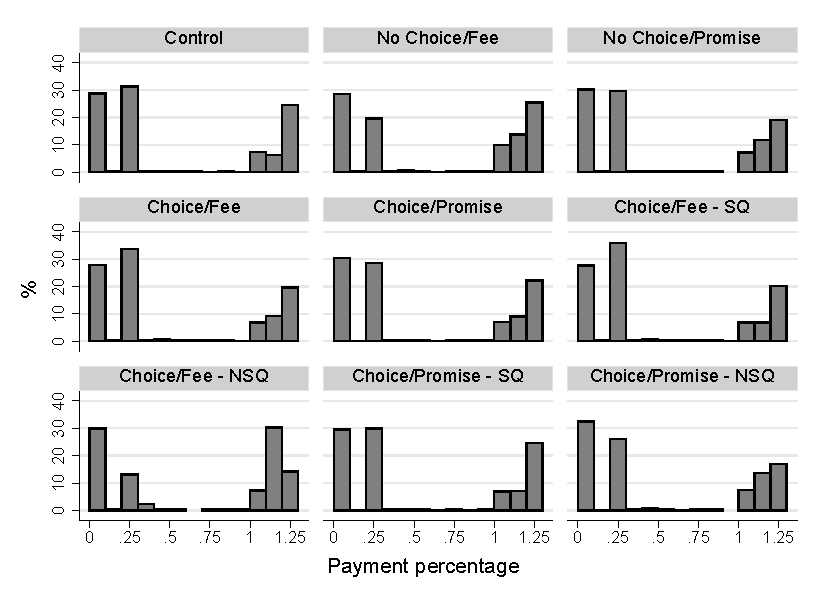
\includegraphics[width=\textwidth]{Figuras/hist_perc_payment.pdf}
    \end{center}
     \footnotesize \textit{Notes: } 
      \footnotesize{ \textit{Do file: }  \texttt{hist\_perc\_payment.do}}
\end{figure}

\pagebreak


%%%%%%%%%%%%%%%%%%%%%%%%%%%%%%%%%%%%%%%%%%%%%%%

% APPENDIX TABLES

\section{APPENDIX}

\subsection{Tables}

\begin{landscape}
\begin{table}[H]
\caption{Treatment effects results}
\label{te_table}
\begin{center}
\scriptsize{% Table generated by Excel2LaTeX from sheet 'te'
\begin{tabular}{rrrrrrrrrrr}
\toprule
      & \multicolumn{2}{c}{} & \multicolumn{2}{c}{} & \multicolumn{2}{c}{} & \multicolumn{2}{c}{} & \multicolumn{2}{c}{} \\
\midrule
\midrule
\multicolumn{1}{l}{} & \multicolumn{2}{c}{(1)} & \multicolumn{2}{c}{(2)} & \multicolumn{2}{c}{(3)} & \multicolumn{2}{c}{(4)} & \multicolumn{2}{c}{(5)} \\
\midrule
\midrule
\multicolumn{1}{l}{No choice/Fee} & \multicolumn{1}{l}{0.11***} & \multicolumn{1}{l}{} & \multicolumn{1}{l}{-5.88*} & \multicolumn{1}{l}{} & \multicolumn{1}{l}{0.076***} & \multicolumn{1}{l}{} & \multicolumn{1}{l}{0.068*} & \multicolumn{1}{l}{} & \multicolumn{1}{l}{0.11***} & \multicolumn{1}{l}{} \\
\multicolumn{1}{l}{} & \multicolumn{1}{l}{(0.023)} & \multicolumn{1}{l}{} & \multicolumn{1}{l}{(3.20)} & \multicolumn{1}{l}{} & \multicolumn{1}{l}{(0.026)} & \multicolumn{1}{l}{} & \multicolumn{1}{l}{(0.038)} & \multicolumn{1}{l}{} & \multicolumn{1}{l}{(0.015)} & \multicolumn{1}{l}{} \\
\multicolumn{1}{l}{No choice/No fee} & \multicolumn{1}{l}{-0.0048} & \multicolumn{1}{l}{} & \multicolumn{1}{l}{-0.30} & \multicolumn{1}{l}{} & \multicolumn{1}{l}{-0.011} & \multicolumn{1}{l}{} & \multicolumn{1}{l}{0.092*} & \multicolumn{1}{l}{} & \multicolumn{1}{l}{0.053***} & \multicolumn{1}{l}{} \\
\multicolumn{1}{l}{} & \multicolumn{1}{l}{(0.022)} & \multicolumn{1}{l}{} & \multicolumn{1}{l}{(3.71)} & \multicolumn{1}{l}{} & \multicolumn{1}{l}{(0.024)} & \multicolumn{1}{l}{} & \multicolumn{1}{l}{(0.051)} & \multicolumn{1}{l}{} & \multicolumn{1}{l}{(0.014)} & \multicolumn{1}{l}{} \\
      &       & \multicolumn{1}{l}{\cellcolor[rgb]{ .929,  .929,  .929} 0.14***} &       & \multicolumn{1}{l}{\cellcolor[rgb]{ .929,  .929,  .929} -6.81*} &       & \multicolumn{1}{l}{\cellcolor[rgb]{ .929,  .929,  .929} 0.097**} &       & \multicolumn{1}{l}{\cellcolor[rgb]{ .929,  .929,  .929} 0.41***} &       & \multicolumn{1}{l}{\cellcolor[rgb]{ .929,  .929,  .929} 0.29***} \\
\multicolumn{1}{l}{Choice/Fee} & \multicolumn{1}{l}{-0.0020} & \multicolumn{1}{l}{\cellcolor[rgb]{ .929,  .929,  .929} (0.037)} & \multicolumn{1}{l}{1.58} & \multicolumn{1}{l}{\cellcolor[rgb]{ .929,  .929,  .929} (3.82)} & \multicolumn{1}{l}{0.0044} & \multicolumn{1}{l}{\cellcolor[rgb]{ .929,  .929,  .929} (0.042)} & \multicolumn{1}{l}{0.10**} & \multicolumn{1}{l}{\cellcolor[rgb]{ .929,  .929,  .929} (0.096)} & \multicolumn{1}{l}{0.029**} & \multicolumn{1}{l}{\cellcolor[rgb]{ .929,  .929,  .929} (0.034)} \\
\cmidrule{3-3}\cmidrule{5-5}\cmidrule{7-7}\cmidrule{9-9}\cmidrule{11-11}\multicolumn{1}{l}{} & \multicolumn{1}{l}{(0.021)} & \multicolumn{1}{l}{\cellcolor[rgb]{ .859,  .859,  .859} -0.018} & \multicolumn{1}{l}{(3.32)} & \multicolumn{1}{l}{\cellcolor[rgb]{ .859,  .859,  .859} 2.89} & \multicolumn{1}{l}{(0.022)} & \multicolumn{1}{l}{\cellcolor[rgb]{ .859,  .859,  .859} -0.0060} & \multicolumn{1}{l}{(0.039)} & \multicolumn{1}{l}{\cellcolor[rgb]{ .859,  .859,  .859} 0.065*} & \multicolumn{1}{l}{(0.013)} & \multicolumn{1}{l}{\cellcolor[rgb]{ .859,  .859,  .859} -0.000012} \\
      &       & \multicolumn{1}{l}{\cellcolor[rgb]{ .859,  .859,  .859} (0.021)} &       & \multicolumn{1}{l}{\cellcolor[rgb]{ .859,  .859,  .859} (3.49)} &       & \multicolumn{1}{l}{\cellcolor[rgb]{ .859,  .859,  .859} (0.022)} &       & \multicolumn{1}{l}{\cellcolor[rgb]{ .859,  .859,  .859} (0.039)} &       & \multicolumn{1}{l}{\cellcolor[rgb]{ .859,  .859,  .859} (0.012)} \\
\cmidrule{9-9}\cmidrule{11-11}      &       & \multicolumn{1}{l}{\cellcolor[rgb]{ .929,  .929,  .929} -0.037} &       & \multicolumn{1}{l}{\cellcolor[rgb]{ .929,  .929,  .929} -8.66**} &       & \multicolumn{1}{l}{\cellcolor[rgb]{ .929,  .929,  .929} -0.058**} &       & \multicolumn{1}{l}{\cellcolor[rgb]{ .929,  .929,  .929} 0.073} &       & \multicolumn{1}{l}{\cellcolor[rgb]{ .929,  .929,  .929} 0.082***} \\
\multicolumn{1}{l}{Choice/No fee} & \multicolumn{1}{l}{-0.0066} & \multicolumn{1}{l}{\cellcolor[rgb]{ .929,  .929,  .929} (0.026)} & \multicolumn{1}{l}{-3.31} & \multicolumn{1}{l}{\cellcolor[rgb]{ .929,  .929,  .929} (4.09)} & \multicolumn{1}{l}{-0.018} & \multicolumn{1}{l}{\cellcolor[rgb]{ .929,  .929,  .929} (0.029)} & \multicolumn{1}{l}{-0.0012} & \multicolumn{1}{l}{\cellcolor[rgb]{ .929,  .929,  .929} (0.057)} & \multicolumn{1}{l}{0.019} & \multicolumn{1}{l}{\cellcolor[rgb]{ .929,  .929,  .929} (0.018)} \\
\cmidrule{3-3}\cmidrule{5-5}\cmidrule{9-9}\cmidrule{11-11}\multicolumn{1}{l}{} & \multicolumn{1}{l}{(0.022)} & \multicolumn{1}{l}{\cellcolor[rgb]{ .859,  .859,  .859} 0.0070} & \multicolumn{1}{l}{(3.43)} & \multicolumn{1}{l}{\cellcolor[rgb]{ .859,  .859,  .859} -1.13} & \multicolumn{1}{l}{(0.023)} & \multicolumn{1}{l}{\cellcolor[rgb]{ .859,  .859,  .859} -0.00055} & \multicolumn{1}{l}{(0.037)} & \multicolumn{1}{l}{\cellcolor[rgb]{ .859,  .859,  .859} -0.035} & \multicolumn{1}{l}{(0.011)} & \multicolumn{1}{l}{\cellcolor[rgb]{ .859,  .859,  .859} -0.010} \\
      &       & \multicolumn{1}{l}{\cellcolor[rgb]{ .859,  .859,  .859} (0.025)} &       & \multicolumn{1}{l}{\cellcolor[rgb]{ .859,  .859,  .859} (3.88)} &       & \multicolumn{1}{l}{\cellcolor[rgb]{ .859,  .859,  .859} (0.026)} &       & \multicolumn{1}{l}{\cellcolor[rgb]{ .859,  .859,  .859} (0.038)} &       & \multicolumn{1}{l}{\cellcolor[rgb]{ .859,  .859,  .859} (0.012)} \\
      &       &       &       &       &       &       &       &       &       &  \\
\multicolumn{1}{l}{Constant (Control)} & \multicolumn{1}{l}{0.44***} & \multicolumn{1}{l}{0.44***} & \multicolumn{1}{l}{92.4***} & \multicolumn{1}{l}{92.4***} & \multicolumn{1}{l}{-0.35***} & \multicolumn{1}{l}{-0.35***} & \multicolumn{1}{l}{0.99***} & \multicolumn{1}{l}{0.99***} & \multicolumn{1}{l}{0.12***} & \multicolumn{1}{l}{0.12***} \\
\multicolumn{1}{l}{} & \multicolumn{1}{l}{(0.015)} & \multicolumn{1}{l}{(0.015)} & \multicolumn{1}{l}{(2.53)} & \multicolumn{1}{l}{(2.53)} & \multicolumn{1}{l}{(0.017)} & \multicolumn{1}{l}{(0.017)} & \multicolumn{1}{l}{(0.028)} & \multicolumn{1}{l}{(0.028)} & \multicolumn{1}{l}{(0.0085)} & \multicolumn{1}{l}{(0.0085)} \\
      &       &       &       &       &       &       &       &       &       &  \\
\midrule
\multicolumn{1}{l}{Observations} & \multicolumn{1}{l}{13446} & \multicolumn{1}{l}{13446} & \multicolumn{1}{l}{6119} & \multicolumn{1}{l}{6119} & \multicolumn{1}{l}{13446} & \multicolumn{1}{l}{13446} & \multicolumn{1}{l}{13446} & \multicolumn{1}{l}{13446} & \multicolumn{1}{l}{13446} & \multicolumn{1}{l}{13446} \\
\multicolumn{1}{l}{R-sq} & \multicolumn{1}{l}{0.007} & \multicolumn{1}{l}{0.010} & \multicolumn{1}{l}{0.003} & \multicolumn{1}{l}{0.005} & \multicolumn{1}{l}{0.003} & \multicolumn{1}{l}{0.005} & \multicolumn{1}{l}{0.002} & \multicolumn{1}{l}{0.006} & \multicolumn{1}{l}{0.010} & \multicolumn{1}{l}{0.028} \\
\multicolumn{1}{l}{Dependent Var Mean} & \multicolumn{2}{c}{0.46} & \multicolumn{2}{c}{90.8} & \multicolumn{2}{c}{-0.34} & \multicolumn{2}{c}{1.04} & \multicolumn{2}{c}{0.16} \\
\midrule
\midrule
\rowcolor[rgb]{ .929,  .929,  .929} Status-quo & \cellcolor[rgb]{ 1,  1,  1}  & \cellcolor[rgb]{ 1,  1,  1}  & \cellcolor[rgb]{ 1,  1,  1}  & \cellcolor[rgb]{ 1,  1,  1}  & \cellcolor[rgb]{ 1,  1,  1}  & \cellcolor[rgb]{ 1,  1,  1}  & \cellcolor[rgb]{ 1,  1,  1}  & \cellcolor[rgb]{ 1,  1,  1}  & \cellcolor[rgb]{ 1,  1,  1}  & \cellcolor[rgb]{ 1,  1,  1}  \\
\rowcolor[rgb]{ .859,  .859,  .859} Non status-quo & \cellcolor[rgb]{ 1,  1,  1}  & \cellcolor[rgb]{ 1,  1,  1}  & \cellcolor[rgb]{ 1,  1,  1}  & \cellcolor[rgb]{ 1,  1,  1}  & \cellcolor[rgb]{ 1,  1,  1}  & \cellcolor[rgb]{ 1,  1,  1}  & \cellcolor[rgb]{ 1,  1,  1}  & \cellcolor[rgb]{ 1,  1,  1}  & \cellcolor[rgb]{ 1,  1,  1}  & \cellcolor[rgb]{ 1,  1,  1}  \\
\end{tabular}%
}
\end{center}
 \footnotesize
\textit{Notes:} 

\textit{Do file: } \texttt{te.do}
\end{table}


\end{landscape}





\subsection{Figures}


\begin{figure}[H]
    \caption{Robustness check effect of arms in reincidence}
    \label{Evolution payment}
    \begin{center}
    \begin{subfigure}{0.49\textwidth}
        \caption{ No Choice/Fee}
        \centering
        \includegraphics[width=\textwidth]{Figuras/reincidence_robust_curve_p2.pdf}
    \end{subfigure}
     \begin{subfigure}{0.49\textwidth}
      \caption*{No Choice/No fee}
        \centering
        \includegraphics[width=\textwidth]{Figuras/reincidence_robust_curve_p3.pdf}
    \end{subfigure}
    
     \begin{subfigure}{0.49\textwidth}
        \caption{Choice/Fee - SQ}
        \centering
        \includegraphics[width=\textwidth]{Figuras/reincidence_robust_curve_p4.pdf}
    \end{subfigure}
     \begin{subfigure}{0.49\textwidth}
      \caption*{Choice/Fee - NSQ}
        \centering
        \includegraphics[width=\textwidth]{Figuras/reincidence_robust_curve_p5.pdf}
    \end{subfigure}
    
    \begin{subfigure}{0.49\textwidth}
        \caption{Choice/No fee - SQ}
        \centering
        \includegraphics[width=\textwidth]{Figuras/reincidence_robust_curve_p6.pdf}
    \end{subfigure}
     \begin{subfigure}{0.49\textwidth}
      \caption*{Choice/No fee - NSQ}
        \centering
        \includegraphics[width=\textwidth]{Figuras/reincidence_robust_curve_p7.pdf}
    \end{subfigure}
    \end{center}
     \footnotesize \textit{Notes: } 
      \footnotesize{ \textit{Do file: }  \texttt{reincidence\_robust\_effect.do}}
\end{figure}


\pagebreak


\begin{figure}[H]
    \caption{Treatment Effect (conditional to positive payment)}
    \label{Treatment Effect}
    \begin{center}
    \begin{subfigure}{0.4\textwidth}
        \caption{Paid loan}
        \centering
        \includegraphics[width=\textwidth]{Figuras/te_graph_des_c_robust.pdf}
    \end{subfigure}
    \begin{subfigure}{0.4\textwidth}
        \caption{Number of payments}
        \centering
        \includegraphics[width=\textwidth]{Figuras/te_graph_num_p_robust.pdf}
    \end{subfigure}
     \begin{subfigure}{0.4\textwidth}
      \caption{Percentage of payment}
        \centering
        \includegraphics[width=\textwidth]{Figuras/te_graph_sum_porcp_c_robust.pdf}
    \end{subfigure}
      \begin{subfigure}{0.4\textwidth}
      \caption{Days to un-pledge}
        \centering
        \includegraphics[width=\textwidth]{Figuras/te_graph_dias_al_desempenyo_robust.pdf}
    \end{subfigure}
    \end{center}
     \footnotesize \textit{Notes: } 
      \footnotesize{ \textit{Do file: }  \texttt{te.do}}
\end{figure}

\begin{figure}[H]
        \caption{Reincidence (conditional to positive payment)}
    \label{micas}
    \begin{center}
        \centering
        \includegraphics[width=\textwidth]{Figuras/te_graph_reincidence_robust.pdf}
    \end{center}
     \footnotesize \textit{Notes: } 
      \footnotesize{ }
\end{figure}



\begin{figure}[H]
    \caption{Evolution of payment}
    \label{Evolution payment}
    \begin{center}
    \begin{subfigure}{0.49\textwidth}
        \caption{Paid loans}
        \centering
        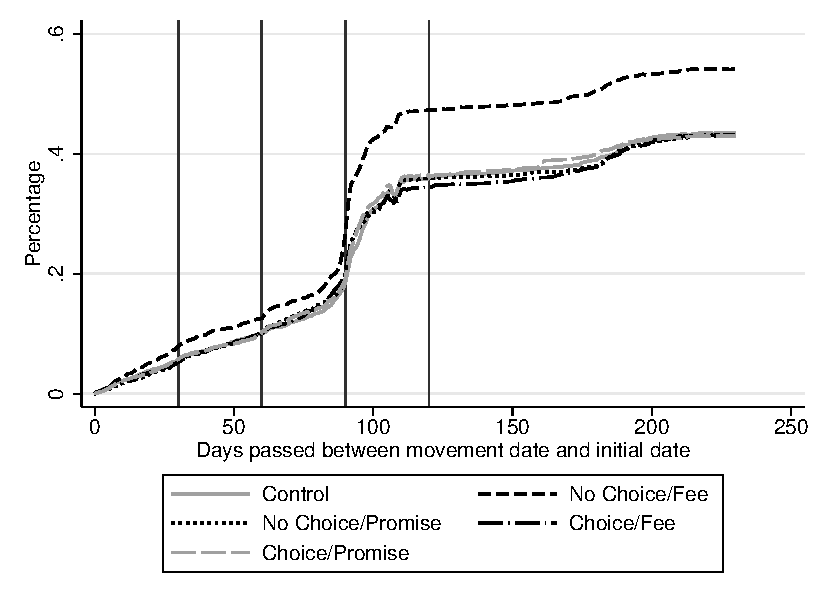
\includegraphics[width=\textwidth]{Figuras/desempeno_evol.pdf}
    \end{subfigure}
     \begin{subfigure}{0.49\textwidth}
      \caption*{}
        \centering
        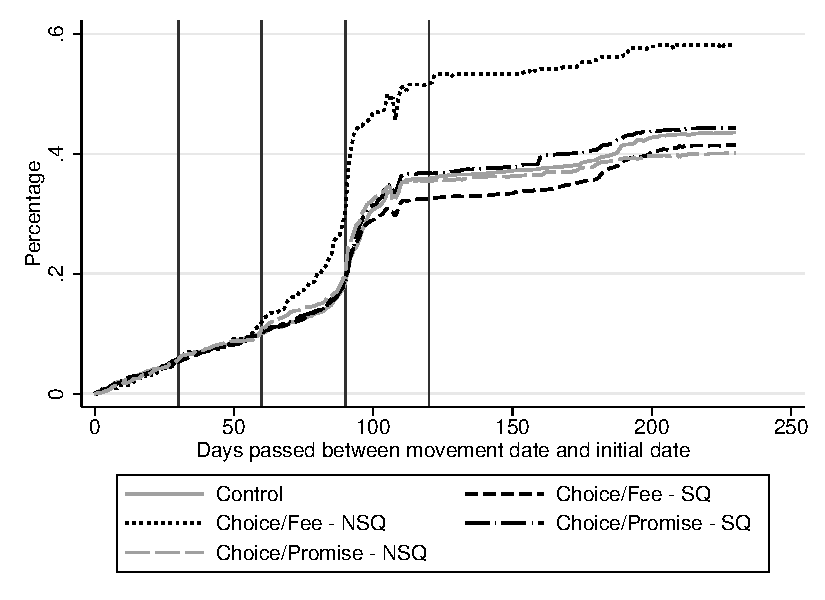
\includegraphics[width=\textwidth]{Figuras/desempeno_evol_choice.pdf}
    \end{subfigure}
    
     \begin{subfigure}{0.49\textwidth}
        \caption{Average percentage of paid loans}
        \centering
        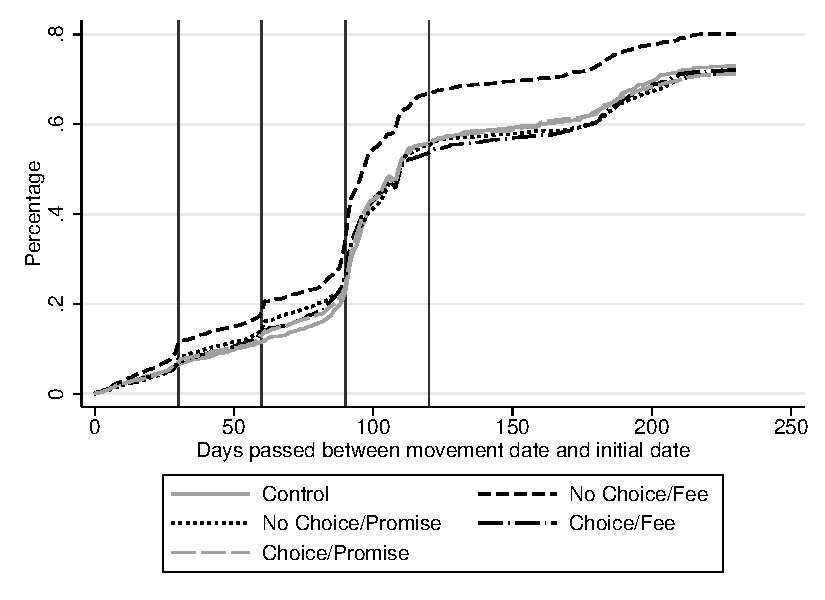
\includegraphics[width=\textwidth]{Figuras/sum_porc_evol.pdf}
    \end{subfigure}
     \begin{subfigure}{0.49\textwidth}
      \caption*{}
        \centering
        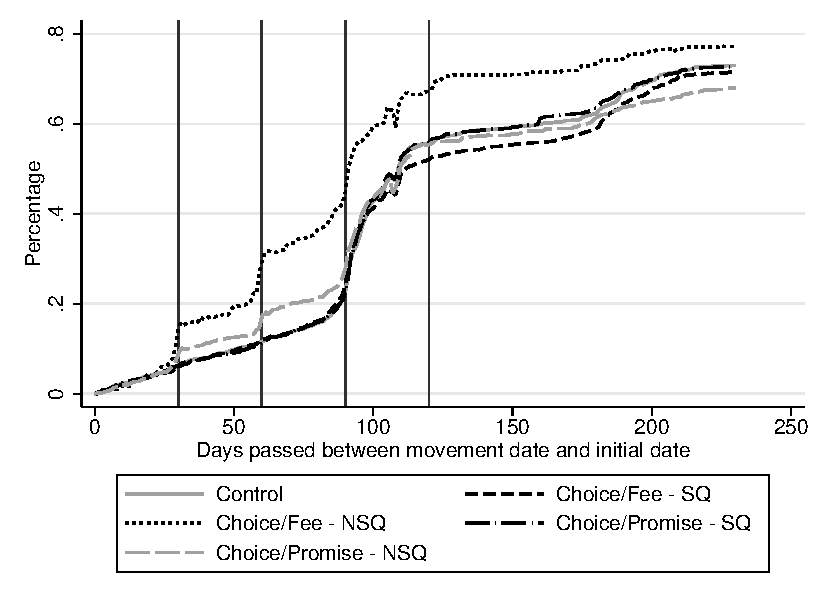
\includegraphics[width=\textwidth]{Figuras/sum_porc_evol_choice.pdf}
    \end{subfigure}
    
    \begin{subfigure}{0.49\textwidth}
        \caption{Average percentage of paid loans (condition on paid loan)}
        \centering
        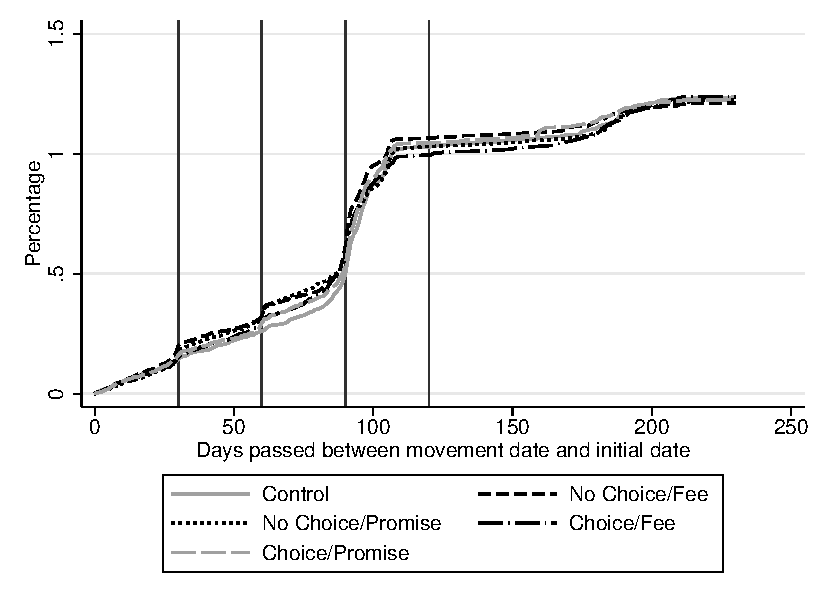
\includegraphics[width=\textwidth]{Figuras/sum_porc_cond_evol.pdf}
    \end{subfigure}
     \begin{subfigure}{0.49\textwidth}
      \caption*{}
        \centering
        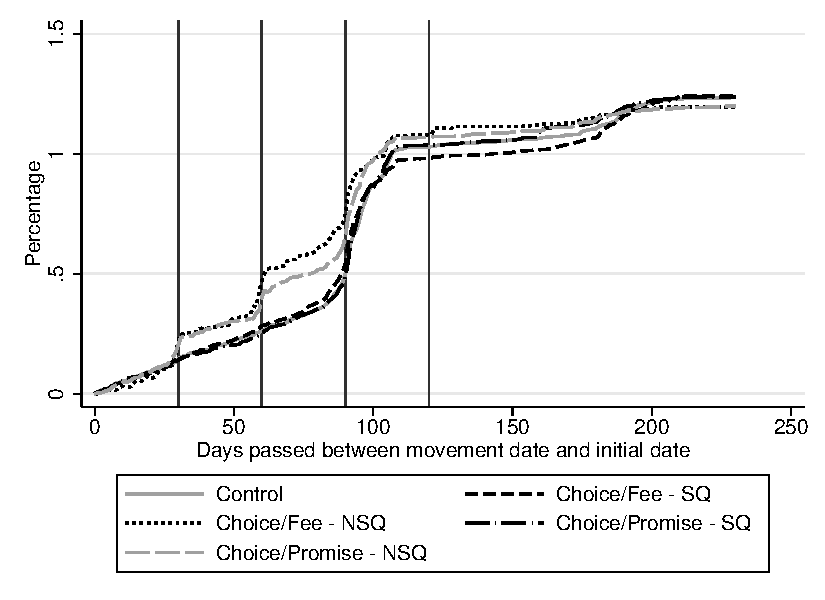
\includegraphics[width=\textwidth]{Figuras/sum_porc_cond_evol_choice.pdf}
    \end{subfigure}
    \end{center}
     \footnotesize \textit{Notes: } 
      \footnotesize{ \textit{Do file: }  \texttt{evol\_payment.do}}
\end{figure}




\end{document}